\section{Y86 Assembly}
\subsection{Process stadier}
Processer kræver instruktioner, der kan organiseres som følgende.
\subsubsection{Fetch}
Her læses bytes for en instruktion, fra hukommelsen.
Dette gøres ved at bruge en Program Counter \textit{PC} som hukommelses addresse.
Disse kaldes \textbf{icode} \textit{(Instruktion kode)} og \textbf{ifun} \textit{(instruktions funktion)}.
En oversigt over disse funktionskoder kan ses i \cref{fig:icode}.
Generelt kan de siges at mængden af bytes der læses, skal adderes til \textit{PC}.
\paragraph{Icode}
Icode gives ved \verb|OP|, altså ved operationen, der udføres.
Rådfør ved \cref{fig:icode}.
\paragraph{Ifun}
Ifun gives ved funktionstypen der udføres. Igen kan der rådføres ved \cref{fig:icode}. 

\subsubsection{Decode}
Her indlæses de givne værdier for funktionen, i \verb|valA| og eller \verb|valB|.
Dette gøres oftest fra \verb|rA| og \verb|rB|, men i nogle tilfælde også \verb|%rsi|.
For instruktioner noteret $\verb|valA|\leftarrow\verb|R[...]|$ er værdien af \verb|R[...]| nummeret på det givne register, der opereres på. Se \cref{tab:y86reg}.

\subsubsection{Execute}
\verb|valE| er værdien, der gives efter \textit{Execute} blokken er kørt.
Her sættes konditions flagene \verb|ZF|, \verb|SF| og \verb|OF|, hvis der skal tjekkes for henholdsvis 0 værdi, negativ værdi eller overflow.
Samtidig noteres operationen som \verb|valx OP valy|.

\subsubsection{Memory}
Her læses eller skrives til computerens hukommelse.

\subsubsection{Writeback}
Her skrives der tilbage, når funktionen er kørt.

\subsubsection{PC update}
Program Counter opdateres.
Her gives værdien af \verb|valP|

\subsection{Registre}
Y86-Assembly har 16 registre til rådighed.
Disse 16 registre vises i \cref{tab:y86reg}
\begin{table}[h]
    \centering
    \begin{tabular}{|l|l||l|l|}
        \hline
        \verb|%rax|&0&\verb|%r8|&8\\
        \verb|%rcx|&1&\verb|%r9|&9\\
        \verb|%rdx|&2&\verb|%r10|&A\\
        \verb|%rbx|&3&\verb|%r11|&B\\
        \verb|%rsp|&4&\verb|%r12|&C\\
        \verb|%rbp|&5&\verb|%r13|&D\\
        \verb|%rsi|&6&\verb|%r14|&E\\
        \verb|%rdi|&7&Intet register&F\\\hline
    \end{tabular}
    \caption{Oversigt over registre i Y86 Assembly}
    \label{tab:y86reg}
\end{table}
Disse registre er næsten alle general purpose, dog med undtagelse af \verb|%rsp|.
\begin{figure}[h!]
    \centering
    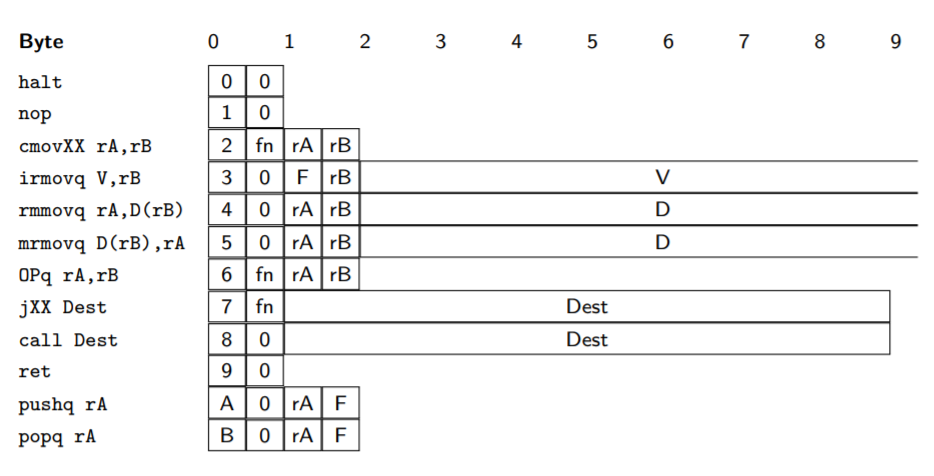
\includegraphics[width=\textwidth]{figures/icodes.png}
    \begin{tabular}{l|c|c||l}
        \hline
        \verb|rrmovq rA, rB|&2&0&Flyt fra register til register\\
        \verb|cmovle rA, rB|&2&1&Flyt hvis mindre eller lig\\
        \verb|cmovl rA, rB|&2&2&Flyt hvis mindre end\\
        \verb|cmove rA, rB|&2&3&Flyt hvis lig med\\
        \verb|cmovne rA, rB|&2&4&Flyt hvis ikke lig\\
        \verb|cmovge rA, rB|&2&5&Flyt hvis større eller lig\\
        \verb|cmovg rA, rB|&2&6&Flyt hvis større end\\\hline
        \verb|addq rA, rB|&6&0&Addition\\
        \verb|subq rA, rB|&6&1&Sutraktion\\
        \verb|andq rA, rB|&6&2&Bitvis AND\\
        \verb|xorq rA, rB|&6&3&Bitvis XOR\\\hline
        \verb|jmp Dest|&7&0&Ikke-konditionelt hop\\
        \verb|jle Dest|&7&1&Hop hvis mindre eller lig\\
        \verb|jl Dest|&7&2&Hop hvis mindre end\\
        \verb|je Dest|&7&3&Hop hvis lig med\\
        \verb|jne Dest|&7&4&Hop hvis ikke lig\\
        \verb|jge Dest|&7&5&Hop hvis større eller lig\\
        \verb|jg Dest|&7&6&Hop hvis større end\\\hline
    \end{tabular}
    \caption{Liste over instruktion- og funktionskoder}
    \label{fig:icode}
\end{figure}
